\chapter{Basics}\label{ch:basics}
    The following chapter provides an overview of research and state-of-the-art in the domain of modelling and simulation of traffic systems.
    Section~\ref{sec:foundational-studies} examines foundational studies that have shaped current understanding of modelling traffic systems, focusing on the methodologies and findings that are most relevant to this thesis.
    Section~\ref{sec:studies-closely-related-to-an-integrated-simulation-environment} focuses on studies that are more closely related to the proposed simulation environment and the challenges that had to be solved in order to create one such integration.
    By mapping out the state of the art, this chapter establishes the context for the subsequent discussion of the proposed approach and methodology in Chapter~\ref{ch:methods}.


    \section{Foundational studies}\label{sec:foundational-studies}
        The field of traffic science is divisible into multiple different sub-categories by the time span of the observed events.
        As described by Treiber et al. \cite{treiber2013traffic} there are vehicle dynamics, traffic flow dynamics and transportation planning as the three major topics(see Table~\ref{tab:dilimination-of-traffic-flow-dynamics}).
        These fields are divisible even further as stated in table~\ref{tab:dilimination-of-traffic-flow-dynamics}.
        The proposed simulation environment would fall into the category of traffic flow dynamics using microscopic car following models.
        According to Treiber et al. this kind of simulation environments are best used to model reaction times, time gaps and the acceleration/breaking behaviors of vehicles in a traffic scenario.
        Driving behavior of vehicles in traffic flow dynamics are usually described by vehicle following (VF) models, which will be discussed further in the following sections.

        \begin{table}[H]
            \centering
            \begin{tabular}{p{.1\linewidth} p{.2\linewidth} p{.2\linewidth} p{.4\linewidth}}
                \hline
                Time scale & Field & Models & Aspects of traffic (examples) \\ \hline \hline
                $\le 0.1 s$ & Vehicle dynamics & Sub-microscopic & Control of engine and breaks \\ \hline
                1 s & \multirow{4}{\linewidth}{Traffic flow dynamics}&\multirow{2}{\linewidth}{Car-following modells} & Reaction time, time gap \\
                10 s & & & Acceleration and deceleration \\\\
                1 min& & \multirow{2}{\linewidth}{Macroscopic models} & Cycle period of traffic lights \\
                10 min & & & Stop-and-go waves \\ \hline
                1 h & \multirow{5}{\linewidth}{Transportation planning} & \multirow{3}{\linewidth}{Route assignment traffic demand} & Peak hour \\
                1 day & & & Daily demand pattern \\
                1 year & & & Building/changing infrastructure \\\\
                5 years & &  \multirow{2}{\linewidth}{Statistics age pyramid} & Socioeconomic structure \\
                50 years & & & Demographic change \\ \hline

            \end{tabular}
            \caption{Delimitation of traffic flow dynamics from vehicular dynamics and transportation planning\cite{treiber2013traffic}}
            \label{tab:dilimination-of-traffic-flow-dynamics}
        \end{table}

        \subsection{Gazis-Herman-Rothery model}\label{subsec:gazis-herman-rothery-model}
            Vehicle following models have been researched for more than 70 years~\cite{pipes1953operational} and many such models have been developed since.
            One of the first widely known VF models is the Gazis-Herman-Rothery (GHR) model (see Eq \ref{eq:GHR}), which described the acceleration of a vehicle $n$ in a driving scenario with respect to the difference in speed $\Delta v$ to the leading vehicle $n-1$ and the distance to the leading vehicle $\Delta x$, at a point earlier in time, with $T$ being the reaction time of the driver\cite{Brackstone1999}.
            \begin{equation}
                a_n(t) = c v_n^m(t) \frac{\Delta v (t-T)}{\Delta x^{-1} (t-T)} \label{eq:GHR}
            \end{equation}

        \subsection{Gipps' model}\label{subsec:gipps-model}
            Gipps states in the paper proposing his own VF model (Gipps´ model), that most VF models up until then (1981) have generally been in the form of EQ~\ref{eq:general-form-vf-model-1981}, where $\tau = T$.
            One example for this general form is the GHR model, some more of those models are found in publications dating back to that time: \cite{newell1961nonlinear, lee1966generalization, bender1970flow}.
            \begin{equation}
                a_n(t+\tau) = l_n \frac{[v_{n-1} - v_n]^k}{[x_{n-1} - x_n]^m}\label{eq:general-form-vf-model-1981}
            \end{equation}
            As pointed out by Philip A. Seddon, the fact, that the time interval between subsequent calculations was given by the reaction time was an undesired characteristic of these models\cite{seddon1972program}, which could be overcome by storing a considerable amount of historical data, which was undesired at the time.
            The second pain point of these models, by today's standards maybe the more relevant point, was the existence of parameters $l_n$,$k$,$m$ (EQ~\ref{eq:general-form-vf-model-1981}), that have no identifiable connection to driver or vehicle characteristics\cite{gipps1981behavioural}.

            To address these deficits, Gipps proposed a new vehicle following model describing the speed of a vehicle at a point in time, in contrast to describing the acceleration of a vehicle at a point in time.
            The following form of the Gipps` model is not the form of the original publication, but the form from~\cite{treiber2013traffic}, which introduces a save speed $v_{save}$ for simplification.
            As stated by Treiber et al. the model is conseptually unchanged.
            The GHR model calculates the speed of a vehicle with respect to the desired acceleration $a$, deceleration $b$, Desired speed $v_0$ and minimum distance $s_0$.
            \begin{align}
                v_{save} (s, v_l) &= -b*\Delta t + \sqrt{b^2 \Delta t^2 - v_l^2 + 2b (s-s_0)} \\
                v(t+ \Delta t) &= min[v+a\Delta t, v_0, v_{save}(s,v_l)] \label{eq:gipps-model-simplified}
            \end{align}
            With the concept of the save speed depending on the distance to the front vehicle $s$ and its speed $v_l$, the gipps` model assembles one of the simplest complete %TODO: explain model completeness
            and accident-free models possible.
            The accident-free characteristic of the model is guaranteed with the assumptions that deceleration and reaction times are constant~\cite{treiber2013traffic}.
            In essence the gipps` model chooses the minimum between the desired speed, the safe speed or the speed that max acceleration would result in the next time step.
            Problem with this model is, that as stated by Treiber et al. it produces an unrealistic acceleration profile.

        \subsection{Intelligent driver model}\label{subsec:intelligent-driver-model}
            The time-continuous Intelligent driver model produces a realistic acceleration profile, since one of the requirements for forming the IDM is that the acceleration function $\dot{v}(s,v,v_l)$ is continuously differentiable in every three variables and thus producing smooth transitions between eg. breaking and acceleration phases.
            Another design criteria of the IDM is that the equilibrium distance\footnotemark has to be larger than the "safe" distance ($v*T + v_0$), with $v$ being the current speed, $T$ being the desired distance between vehicles in seconds and $v_0$ representing the "bumper-to-bumper" distance (min distance kept between vehicles), which ensures the accident-free characteristic of that model.
            \footnotetext{The Distance, that is required between vehicles to stay in a steady-state equilibrium, which means, in a homogenous convoy the distance between all vehicles and the speed is the same.
            Furthermore, the acceleration has to be 0 for every vehicle to be in a steady-state eqilibrium. \cite{treiber2013traffic, treiber2000IDM} }

            \begin{align}
                s^*(v,\Delta v) = s_0 + \max\left( 0, vT + \frac{v \Delta v}{2 \sqrt{ab}} \right) \label{eq:IDM-s-star} \\
                \dot{v}(s,v,v_l) = a * \left[ 1- \left(\frac{v}{v_0}\right)^\delta  - \left( \frac{s^*(v, \Delta v)}{s} \right)^2\right] \label{eq:IDM}
            \end{align}

            The IDM (see EQ~\ref{eq:IDM})is constructed from 2 pieces, the first part is comparing the current speed to the desired speed: $\left(\frac{v}{v_0}\right)^\delta$.
            The second part is comparing the current distance to the desired distance $s^*$ (see EQ~\ref{eq:IDM-s-star}): $\left( \frac{s^*(v, \Delta v)}{s} \right)^2$~\cite{treiber2013traffic, treiber2000IDM}.

            The advantage of using an intuitive model like Gipps` model or the IDM, is that they are easy to configure by some simple understandable parameters (including vehicle and driver specific numbers).
            For example the configuration of the IDM consists of six parameters controlling the behavior of vehicles, with default values used by TraffSim (see Table~\ref{tab:IDM-Default-Values})~\cite{treiber2013traffic,backfrieder2013traffsim,backfrieder2014traffsim}.
            The Implementation in TraffSim includes two additional parameters, determining the maximum possible acceleration $a_{max}$ and deceleration $b_{max}$, which act as a hard limit for the acceleration function.
            The value of $b_{max}$ for example models the physical limit of the breaks of a car.
            \begin{table}[H]
                \centering
                \begin{tabular}{l c c}
                    Parameter & TraffSim default Value & Acceptable Range \\
                    \hline
                    Comfortable acceleration $a$ & $2 \si{\m\per\s\squared}$ & $ 0 < a < a_{max}$\\
                    Comfortable deceleration $b$ & $-2 \si{\m\per\s\squared}$ & $ b_{max} < b < 0$\\
                    Desired Speed $v_0$ & $25 \si{\m\per\s}$ & $v_0 > 0$ \\
                    Minimum bumper-to-bumper distance $s_0$ & $2 \si{\m}$ & $s_0 > 0$ \\
                    Time gap $T$ & $1.5 \si{\s}$ & $T > 0$\\
                    Acceleration exponent $\delta$ \footnotemark& 4 & $\delta >  0$\\
                \end{tabular}
                \caption{Default Values for IDM}
                \label{tab:IDM-Default-Values}
            \end{table}
            \footnotetext{Dimensionless factor determining the rate at wich the vehicle`s acceleration decreases as it approaches its desired velocity}

        \subsection{Micro traffic simulation}\label{subsec:micro-traffic-simulation}
                The aforementioned vehicle following models are an integral part of a traffic simulator as they are used to control the movement of vehicles along the road network.
                Since one such simulator is a key building block of the desired simulation environment, the next section focuses on the micro traffic simulation environments available in literature.
                Special focus will be placed onto the micro traffic simulator TraffSim~\cite{backfrieder2013traffsim,backfrieder2014traffsim}, developed in house at Hagenberg.
            \subsubsection{MovSim}
                The first notable example is MovSim~\cite{Treiber2010}, which is an open source, free to use traffic simulator developed by a team at TU Dresden.
                MovSim implements the IDM (see Section~\ref{subsec:intelligent-driver-model}) among other vehicle following model which is responsable for the longitudinal movement of vehicles.
                For transversal movement of vehicles, MovSim utilizes the MOBIL model~\cite{kesting2007general}, which is a model for lane changing working alongside a variety of VF models.
                MovSim is primary source for sample implementations of VF models described by Treiber et al. (in~\cite{treiber2013traffic}).
                A picture of the web based user interface is depicted in Figure~\ref{fig:mov-sim-ui}.

                \begin{figure}[H]
                    \centering
                    \includegraphics[width=0.7\textwidth]{Movsim}
                    \caption{MovSim user interface~\cite{MovSimUI}}
                    \label{fig:mov-sim-ui}
                \end{figure}
            \subsubsection{Eclipse SUMO}
                One of the most popular traffic simulation environments is Eclipse SUMO~\cite{Behrisch2011SUMOS}, which is a suite of applications to model and simulate traffic scenarios.
                SUMOs development started in 2001 and has been made publicly available and open source in 2002.
                The simulation suite includes two applications used to import/generate road networks from a variety of sources.
                \begin{enumerate}
                    \item \textit{netgen}: The \textit{netgen} tool is able to generate a fictional road network based on a set of input parameters.
                        Different kinds of road networks can be generated by \textit{netgen}: Grid Networks, Spider Networks and Random networks~\cite{SUMOWebsite}.
                    \item \textit{netconvert}: This tool converts a road network, described by a variety of input formats, into a SUMO usable road network.
                        Among other input file formats, netgen supports road networks from other simulators like Vissim~\cite{lownes2006vissim} or MATsim~\cite{balmer2009matsim,w2016multi}.
                        Furthermore, the importing filetypes like OpenStreetMap~\cite{haklay2008openstreetmap} and OpenDRIVE~\cite{openDrive} is supported~\cite{Behrisch2011SUMOS}.
                \end{enumerate}
                Many other applications are part of the SUMO suite that can be used for e.g. modelling V2X vehicles, generating routes from inputs like Source/Destination matrices or Loop detector statistics~\cite{Behrisch2011SUMOS}.
                SUMO can be used in command-line mode for efficient simulation of a large number of parallel scenarios or in graphical UI mode for viewing a simulation while running (see Figure~\ref{fig:sumo-UI}).
                During the runtime of simulations its possible to record statistics, that can be analyzed in post-processing.

                \begin{figure}[H]
                    \centering
                    \includegraphics[width = 0.7\textwidth]{SUMO_UI}
                    \caption{"Screenshot of the graphical user interface coloring vehicles by
                    their CO2 emission."\cite{Behrisch2011SUMOS}}
                    \label{fig:sumo-UI}
                \end{figure}
        \subsubsection{TraffSim}
            TraffSim is a microscopic traffic simulator develeoped by a Team at University of Applied Scieneces Upper Austria.
            It`s initial purpose, was to investigate the impact of intelligent traffic management on traffic flow, by using V2V-technology to dynamically reroute vehicles and thus reduce traffic jams.
            Since then TraffSim has gone through a major rewrite and getting the name TraffSim-B.
            TraffSim-A has been an Application developed in Java with a conventional desktop GUI, whereas TraffSim-B switched to Spring Boot\cite{walls2015spring} and Vaadin\cite{gronroos2009book} as its Frontend, thus the new version is used in a web browser.
            The following work, if not otherwise stated, is referring to the TraffSim-B version.

            TraffSim is built to use OpenStreetMap data as input for its road network, which is loaded and transformed into a working Scenario.
            To allow for computation of routes, a directed weighted cyclic graph is generated, that enables TraffSim to use a pathfinding Algorithm\cite{foead2021systematic}.
            Furthermore, the road network is transformed into TraffSims own datastructures, using SUMOs \textit{netconvert} tool.
            The transformed network is then stored into a local MongoDB instance
            In figure~\ref{fig:traffSim-road-network} the datastructures, used in TraffSim, to store the Road Network are visualized.
            In essence, a RoadSemgnet consists of one or more LaneSegments.
            RoadSegments can be connected directly to each other (1:1) or by a Junction.
            One such junction consists therefor of one or more Junction Connectors.
            Any DrivableArea is represented by the width and a reference line, which is composed of multiple points that are connected by straight lines.
            Which implies, that turns in the road network are also represented by small straight segements and thus do not appear to be smooth.
            The consequences of this will be discussed in more detail in Section %TODO: problem mit straßennetzrepresentation Chapter.

            \begin{figure}[H]
                \centering
                \begin{tikzpicture}[node distance=2cm]
                    % Classes
                    \node (Segment) [class] {Segment};
                    \node (RailSegment) [class, below left of=Segment, xshift=-1.5cm] {RailSegment};
                    \node (RoadSegment) [class, below right of=Segment, xshift=1.5cm] {RoadSegment};
                    \node (DrivableArea) [class, below of=Segment, yshift=-1.5cm] {DrivableArea};
                    \node (LaneSegment) [class, below left of=DrivableArea, xshift=-1.5cm] {LaneSegment};
                    \node (JunctionConnector) [class, below right of=DrivableArea, xshift=1.5cm] {JunctionConnector};

                    % Arrows (Inheritance relationships)
                    \draw [arrow] (RailSegment) -- (Segment);
                    \draw [arrow] (RoadSegment) -- (Segment);
                    \draw [arrow] (DrivableArea) -- (Segment);
                    \draw [arrow] (LaneSegment) -- (DrivableArea);
                    \draw [arrow] (JunctionConnector) -- (DrivableArea);

                \end{tikzpicture}
                \caption{Class diagram of road network representation in TraffSim}
                \label{fig:traffSim-road-network}
            \end{figure}

            The position of vehicles, moving along the road network, are represented by the DrivableArea they are on and by the distance, along the current segment, of their front relative to the start of the Segment.
            This implies, that vehicles in TraffSim esentially behave like trains on a railroad moving only longitudinal along the street and having no latitudinal movement.

            TraffSim belongs to the class of time-discrete simulation environments, meaning, all changes in simulation state changes at an explicit point in time.
            The vehicle following models implemented in TraffSim are mostly given in time-continuous form, modelling the acceleration $a_\alpha$ of a vehicle $\alpha$ \cite{TraffSimDoku}.
            These time-continuous models have to be augmented by a numerical integration technique for usage, calculating the resulting speed and distance traveled by the vehicle with the newtonian equations of movement.
            Multiple algorithms are valid candidates for usage in traffic simulations according to~\cite{treiber2015comparing} the default method for numerical integration of Ordinary Differential Equations (like the newtonian equations of movement) is the fourth order Range-Kutta scheme).
            For example the Range-Kutta integration scheme is used in.
            Although Range-Kutta is used in some examples like~\cite{kaupuvzs2004applications, shamoto2011car}, most simulators implement a simpler approach or do not state the used numerical integration at all\cite{treiber2015comparing}.
            Commonly either Euler`s method is used for integration (e.g used in AIMSUN~\cite{casas2010traffic} or Eclipse SUMO~\cite{Behrisch2011SUMOS}).
            Or a ballistic approach is used, this means, the acceleration during calculation of a subsequent timestep is assumed constant.
            This ballistic method is implemented in TraffSim, which results in the following calculations for speed $v_\alpha$ (see Equation~\ref{eq:numerical-integration-v})and position on the road $s_\alpha$ (see Equation~\ref{eq:numerical-integration-s})~\cite{TraffSimDoku}.

            \begin{figure}
                \centering
                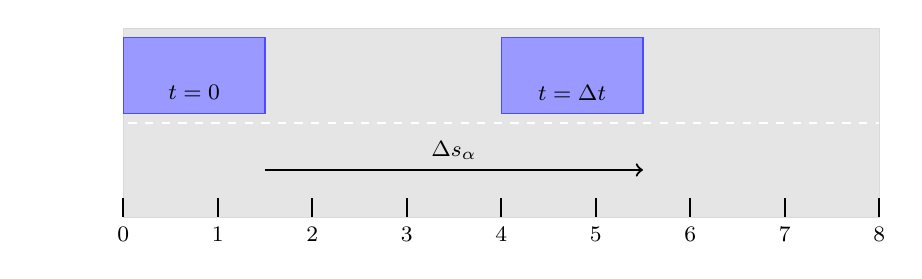
\begin{tikzpicture}[scale=1.2, every node/.style={font=\footnotesize}]
                    \draw[gray!30, fill=gray!20] (0,-1) rectangle (8,1);
                    \draw[white, dashed, thick] (-1,0) -- (8,0);
                    \foreach \x in {0,1,...,8}
                    \draw[black, thick] (\x, -0.8 ) -- (\x,-1) node[below]{\x};
                    % Position 1 (t=0): Vehicle
                    \draw[blue!70, fill=blue!40] (0,0.1) rectangle (1.5,0.9) node[black,midway, below]{$t = 0$};

                    % Position 2 (t=1): Vehicle
                    \draw[blue!70, fill=blue!40] (4,0.1) rectangle (5.5,0.9) node[black,midway, below]{$t = \Delta t$};
                    \draw[->, thick] (1.5,-0.5) -- (5.5,-0.5) node[midway, above]{$\Delta s_\alpha$};
                \end{tikzpicture}
                \caption{Example of vehicle position update}
                \label{fig:traffsim-veh-pos-update}
            \end{figure}

            \begin{align}
                v_{\alpha}(t + \Delta t) &= v_{\alpha}(t) + a_\alpha(t) * \Delta t \label{eq:numerical-integration-v} \\
                s_{\alpha}(t + \Delta t) &= s_{\alpha}(t) + v_{\alpha}(t) * \Delta t + \frac{1}{2} v_{\alpha}(t) * (\Delta t)^2 \label{eq:numerical-integration-s}
            \end{align}

            This distance calculated is than added to the vehicles position on the road.
            If the calculated distance added to the vehicles current position is less than the road length it is simply added, if it is greater, the vehicle is placed on the next road segment of the route.
            In the example shown in Figure~\ref{fig:traffsim-veh-pos-update}, a Vehicle is at time $t=0$ at position $s=1.5$ on the road, in the next time step, the Vehicle moves by $\Delta s_\alpha$.
            By doing this process over and over again, the Vehicles are "driving" along the roadnetwork in TraffSim.


            The architecture of TraffSim (see Figure~\ref{fig:traffSim-architecture}) is designed, that a great number of simulations, from the same scenario or different, can be run in parallel.
            Therefor TraffSim strictly separates the logic during a Simulation from the input data describing the Scenario.
            For each Scenario the input data is kept in the Simulation Model, which is stored in the local MongoDB instance.
            "It contains all the entities that are configurable, which include the road network, the route graph, repositories for (e.g. vehicles, routes, RSUs\footnote{Road Side Units}), traffic generators and much more"~\cite{TraffSimDoku}.
            Every Simulation Run\footnote{A SimulationRun is a running instance of a Scenario} gets a copy of the Simulation Model, that is used to carry out the simulation.
            Since the model is copied into every instance, the same scenario can be run multiple times in parallel.
            This is especially useful when using batch simulations, which allow the user to vary parameters and investigate the impact of one/many parameter variations onto the traffic.
            Since it`s impractical to visually track multiple simulations, when using batch mode the UI is disabled and just the statistics are generated and can be analyzed in post processing.
            The Statistics are exported using the HDF (.h5) file format and can be analyzed in Matlab or Python using the, in TraffSim included, libraries.

            \begin{figure}[H]
                \centering
                \includegraphics[width=\textwidth]{TraffSimArchitecture}
                \caption{TraffSim Archtecture\cite{TraffSimDoku}}
                \label{fig:traffSim-architecture}
            \end{figure}

            The control logic of many features of TraffSim is implemented in Time Step Divers, which is a mechanism inside TraffSim that allows the developer to register Components that get called repeatedly during the simulation.
            This could eiter be a fixed time interval (in simulation time) or during the calculation of every simulation step.
            There is a defined order, in wich the individual Time Step Drivers are called.
            One notable example of one such Time Step Driver is the SimulationUpdater, this module invokes the calculation of the acceleration of every vehicle on the RoadNetwork using its associated vehicle following models.

        \subsection{Driving simulation}\label{subsec:driving-simulation2}
            Driving simulators and traffic simulators follow distinct but complementary objectives within the broader field of transportation research.
            While traffic simulators generally focus on modeling the aggregate or microscopic flow of vehicles across a network, driving simulators emphasize individual driver experience, behavior, and interaction with the vehicle or environment.
            This section delineates the main differences between these two categories of simulation tools and highlights reasons why both are integral to modern transportation research.

            \subsubsection{Level of Abstraction}
                In the category of traffic simulators, as discussed earlier, there are different levels of detail in simulations: microscopic-, mesoscopic- and macroscopic simulation.
                Where each of these kind of simulators adds a layer of abstraction, from microscopic models, tracking each vehicle and the interaction with others to macroscopic models, which represent the flow of vehicles as continuous fluid-like streams.
                Driving simulators are located somewhere below the microscopic traffic simulators, because they are modeling one vehicle`s physical properties and behavior to a great extent.
                For example, a traffic simulator usually reduces the model of a vehicle`s engine to some primitive parameters like max acceleration and efficiency, a driving simulator models the engine in much greater detail, including torque curves, power curves and many more engine specific parameters.
                In contrast to most traffic simulators, driving simulators do allow lateral movement of vehicles on the road.
                That means, that vehicles are not only bound to the center of the lane but are able to move free in 3 dimensions.

            \subsubsection{Fidelity and Realism}
                Driving simulators are designed to deliver realistic visual and physical environments.
                Many use game engines or high-end graphics libraries to simulate lighting, weather conditions, and road surfaces with high fidelity.
                Some simulators also support hardware-in-the-loop (HIL) configurations, which utilize real steering wheels, pedals, and motion platforms to replicate the physical sensations associated with driving~\cite{sievers2018driving}.
                These features are essential for various research applications, including human factors studies, driver assistance testing, and the prototyping of autonomous vehicle algorithms that depend on camera or LiDAR\cite{collis1970lidar} data.

                In contrast, traffic simulators typically utilize simplified graphical interfaces or purely abstract representations of road networks~\cite{Treiber2010}.
                While visualization has evolved over time, it continues to prioritize monitoring flow patterns, such as queue formation or travel-time distributions, over replicating photorealistic driving experiences~\cite{carla2017}.

            \subsubsection{Driver in the loop}
                Driving simulators typically enable driver-in-the-loop experiments, in which a human or advanced AI driver interacts with the virtual environment in real time.
                This setup is vital for evaluating driver behavior under different road, traffic, or weather conditions and for testing advanced driver-assistance systems (ADAS) before deployment.
                Such real-time interactions yield deeper insights into cognitive and perceptual aspects that standard offline simulations can overlook.
                Coupled with advanced data collection techniques, it becomes possible to measure factors such as driver workload, reaction times, and overall situational awareness.
                In addition, driver-in-the-loop experiments provide a controllable environment for investigating emergency braking maneuvers, crash avoidance strategies, and the human–machine interface in partially automated vehicles~\cite{riener2017driver, riegler2023}.


            \subsubsection{CARLA}
                In addition to some other notable examples like Madras~\cite{santara2021madras} or Torcs~\cite{wymann2000torcs}, CARLA~\cite{carla2017} is a free to use and open source driving simulator.
                CARLA is built using the widely adopted Unreal Engine~\cite{lewis2002game} and thus developed in the programming language C++.
                The simulator is available on Windows and Linux as desktop application.
                CARLA is designed in a classical Client-Server architecture, as depicted in Figure~\ref{fig:carla-architecture}, a server is started and multiple clients can be connected to one such server.
                Typically, these clients are implemented in Python, since CARLA provides a feature rich API Library to interact with it`s server.
                When starting the carla Server one is provided a game window with a camera that is movable through the game world.
                The actual vehicle control has to be done via a python client application, there are some default examples for such client programs.
                The key advantage of this architecture is, that CARLA can be used in a vast variety of scenarios, the vehicles in the simulation can be controlled by humans, machine learning algorithms~\cite{liu2022synthetic}, static pathfinding algorithms or for example by real world vehicles in need for a digital twin~\cite{steinmetz2022digital}.
                A common use case of carla is to train neuronal networks to control a vehicle in the simulation environment~\cite{Codevilla2019, ramosautonomous}.

                \begin{figure}[H]
                    \centering
                    \includegraphics[width=0.8\textwidth]{Carla-Simulator-System-Architecture-Pipeline}
                    \caption{Carla client-server architecture \cite{pirri2021towards}}
                    \label{fig:carla-architecture}
                \end{figure}

    \section{Studies closely related to an integrated simulation environment}\label{sec:studies-closely-related-to-an-integrated-simulation-environment}
        \subsection{OpenDrive/OpenScenario}\label{subsec:opendrive/openscenario}
            OpenDRIVE and OpenSCENARIO represent complementary standards for modeling and exchanging data in traffic simulation and autonomous driving research (see Figure~\ref{fig:openDRIVE-overview}).
            OpenDRIVE focuses on the precise description of road networks, including lane geometry, signage, and signal systems, while OpenSCENARIO targets the definition of traffic maneuvers, actor behaviors, and event sequences.
            Together, these formats enable consistent scenario creation and simulation across different software platforms, thereby reducing integration challenges and facilitating reproducible experiments.
            Through standardized road network specification and scenario scripting, researchers and developers can more efficiently collaborate on validation efforts for automated driving systems.
            These Standards use XML Files to represent data of road networks and driving maneuvers, the files are typically using the file ending ".xodr".


            \begin{figure}[H]
                \centering
                \includegraphics[width=.8\textwidth]{open_drive_open_scenario}
                \caption{Relationship between OpenDRIVE and OpenSCENARIO~\cite{openDrive}}
                \label{fig:openDRIVE-overview}
            \end{figure}

            An OpenDRIVE file mainly consists of Junctions and Roads, described by the Listing~\ref{lst:xodr-file} is a example of a described road in OpenDRIVE format.
            As visible from the example file, a road is modelled by many parameters like id, name, length, predecessor, successor, ....
            The tags "<planView>", "<lane>" and "<elevationProfile>" will be discussed in the following sections.
                
            \begin{minipage}{\textwidth}
            \begin{GenericCode}[caption={Example OpenDRIVE File~\cite{carlaGit}}, label={lst:xodr-file}]
road name="Road 0" length="3.95e+1" id="0" junction="-1">
    <link>
        <predecessor elementType="junction" elementId="106"/>
        <successor elementType="junction" elementId="281"/>
        </link>
            <type s="0.00e+0" type="town">
                <speed max="55" unit="mph"/>
            </type>
        <planView>
            <geometry s="0.00" x="2.11e+2" y="3.09e+2" hdg="-1.02e-2" length="3.95e+1">
                <line/>
            </geometry>
        </planView>
        <elevationProfile>
            <elevation s="0.00e+0" a="4.34e-3" b="0.00e+0" c="0.00e+0" d="0.00e+0"/>
        </elevationProfile>
        <lanes>
            <laneOffset s="0.00e+0" a="0.00e+0" b="0.00e+0" c="0.00e+0" d="0.00e+0"/>
            <laneSection s="0.000+0">
                <left>
                    <lane id="1" type="driving" level="false">
                        <width sOffset="0.00e+0" a="3.50e+0" b="0.00e+0" c="0.00e+0" d="0.00+0"/>
                        <roadMark sOffset="0.00e+0" type="none" material="standard" color="white" laneChange="none"/>
                        <roadMark sOffset="6.12e+0" type="solid" material="standard" color="white" width="1.25e-1" laneChange="none"/>
                        <userData>
                            <vectorLane travelDir="backward"/>
                        </userData>
                    </lane>
                </left>
                <center>
                    <lane id="0" type="none" level="false">
                        <roadMark sOffset="0.00e+0" type="none" material="standard" color="white" laneChange="none"/>
                        <roadMark sOffset="6.12e+0" type="broken" material="standard" color="yellow" width="1.25e-1" laneChange="none"/>
                    </lane>
                </center>
                <right>
                </right>
            </laneSection>
        </lanes>
    </road>
                \end{GenericCode}
                \end{minipage}

            \subsubsection{Reference line system}

                \begin{figure}[H]
                   \centering
                   \includegraphics[width=\textwidth]{reference_line_system}
                   \caption{Reference Line System \cite{openDrive}}
                   \label{fig:ref-line-sys}
                \end{figure}
                As depicted in the Figure~\ref{fig:ref-line-sys}, a road is modelled in 3 Layers.
                \begin{enumerate}
                    \item Reference line \textit{<planView>}: The course of a road segment is described by a line in the center of the Road.
                        Since the curse of roads can have a variety of shapes, this line can be described with one of the following geometric elements\cite{openDrive}:
                        \begin{itemize}
                            \item Straight line
                            \item Spirals
                            \item Arcs with constant curvature
                            \item Parametric cubic polynomials
                            \item Cubic polynomials
                        \end{itemize}
                        This reference line is always placed at the base plane of the map.
                        Therefore, it describes the road in 2 Dimensions, the elevation profile of the road is modelled by usage of the \textit{<elevationProfile>} tag, that describes the elevation of a road segment using a 3rd order polynomial.
                        Any mix of the geometric elements can be used to describe any possible course of a road as depicted in Figure~\ref{fig:opendrive-geom}.
                        \begin{figure}[H]
                            \centering
                            \includegraphics[width=.8\textwidth]{opendrive_reference_line_geom}
                            \caption{Combined geometrics~\cite{openDrive}}
                            \label{fig:opendrive-geom}
                        \end{figure}
                    \item Lane \textit{<lane>}: One road can have multiple lanes on the right and left side, with each lane having an identifier.
                        The lanes to the right of the center line are identified by negative numbers and the lanes on the left side with positive numbers.
                        Lanes are added along the reference line and thus make the infinitely thin line into a surface with specific length and width.
                        In addition to the width, lanes can be decorated with road markings.
                    \item Features: A modelled road can be enhanced with additional features like speed limits, traffic signals, etc.
                \end{enumerate}
            For editing and viewing of openDRIVE files, tools like OpenDRIVE viewer (\url{https://odrviewer.io/}) or Mathworks` RoadRunner can be used.
            OpenDRIVE is also utilized by CARLA to import road networks into scenarios.

        \subsection{Map matching}\label{subsec:basics-map-matching}
            Map matching is the process of aligning observed vehicle positions, typically recorded via GPS or other location-tracking sensors, to the correct roads or paths on a digital map.
            This step is essential in navigation, route planning, and autonomous driving applications, as it mitigates positioning errors and ensures that location data remain consistent with the underlying road network~\cite{huang2021survey}.
            Various methodologies, including topological~\cite{white2000some, joshi2001new, greenfeld2002matching}, geometric~\cite{bernstein1996introduction}, and probabilistic approaches~\cite{Quddus2006}, have been proposed to address different accuracy and computational demands~\cite{quddus2007current}.
            By anchoring vehicle positions to a known map, map matching facilitates reliable trajectory tracking, route deviation detection, and sensor fusion for advanced driver assistance systems.

            In the field of geometric map matching algorithms, 3 categories can be distinguished:
            \begin{enumerate}
                \item Point-to-Point matching: the most straight forward way of matching an arbitrary position to a road network would be to find the closest node of the network.
                    In most cases the Euclidean distance (see Equation~\ref{eq:euclidian-distance}), usually in $\mathbb{R}^2$, is used to determine the closest node, by iteratively checking the given position with each node of the road network and storing the lowest value~\cite{bernstein1996introduction}.
                    \begin{equation}
                        d(p,q) = \sqrt{ (p_0 - q_0)^2 + (p_1 - q_1)^2  + \hdots  + (p_n - q_n)^2}
                        \label{eq:euclidian-distance}
                    \end{equation}
                    This method works well when the road network consists of lots of nodes and the connection between those nodes are fairly short.
                    If dealing with long straight roads, the method stops working.
                \item Point-to-Curve matching: To conquer the mentioned problem, one might attempt to find the road segment $N$ nearest to the given position instead of searching for the nearest node.
                    In order to calculate the minimum distance of a point $p$ to a road, the distance to each line segment $A$ of the road has to be computed.
                    Using Equation~\ref{eq:distance-to-line} (Line $A$ is described by its Endpoints $a$ and $b$), the minimum perpendicular distance between $p$ and $A$ can be calculated (see Figure~\ref{fig:point-to-curve-matching},blue case)~\cite{bernstein1996introduction}.
                    \begin{equation}
                        d_{line}(p,A) = \sqrt{\frac{((a_y-b_y)*c_x+(b_x-a_x)*c_y + (a_x*b_x - b_x*a_y))^2}{(a_y-b_y)^2 + (b_x-a_x)^2}}
                        \label{eq:distance-to-line}
                    \end{equation}

                    If the intersection $q$ of the perpendicular line of $p$ and $A$ is be not between $a$ and $b$ (see Figure~\ref{fig:point-to-curve-matching}, red case), the minimum distance of between $(p,a)$ and $(p,b)$ is taken as distance to the line~\cite{bernstein1996introduction}.
                    \begin{equation}
                        D(p,A) = \begin{cases}
                            d_{line}(p, A) &  \max(d(q,a), d(q,b)) < d(a,b) \\
                            \min(d(p,a) , d(p,b)) & otherwise
                        \end{cases}
                    \end{equation}
                    \begin{figure}[H]
                        \centering
                        \begin{tikzpicture}[
                            scale=1.2,
                            line cap=round,
                            line join=round,
                            >=Stealth,
                            every node/.style={font=\small}
                        ]
                            % Define two main points for the black line
                            \coordinate (A0) at (0,0);
                            \coordinate (A1) at (4,0);
                            \coordinate (p1) at (2, -1);
                            \coordinate (q1) at (2, 0);
                            \coordinate (p2) at (-1, -1);
                            \coordinate (q2) at (-1,0);

                            \filldraw[black] (p1) circle (1.5pt);
                            \filldraw[black] (q1) circle (1.5pt);
                            \filldraw[black] (p2) circle (1.5pt);
                            \filldraw[black] (q2) circle (1.5pt);
                            \filldraw[black] (A0) circle (1.5pt);
                            \filldraw[black] (A1) circle (1.5pt);

                            % Draw the main black line
                            \draw[thick] (A0) -- (2,0)node[above]{$A$} -- (A1);
                            % Extend the dashed line beyond A0 and A1
                            \draw[dashed] ((-1.5,0) -- (5.5,0));

                            % Draw red dotted segment from A0 to q
                            \draw[blue] (p1) -- (2,-0.5) node[right]{$D(A,p_1)$} --  (q1);
                            \draw[red] (p2) -- (-0.5, -0.5) node[right]{$D(A,p_2)$} -- (A0);
                            \draw[dotted] (2,0) -- (A1);
                            \draw[dotted] (p2) -- (-1,0.2);

                            % Label the points
                            \node[above left]  at (A0) {\(a\)};
                            \node[above right] at (A1) {\(b\)};
                            \node[below left]  at (p1)  {\(p_1\)};
                            \node[below left]  at (p2)  {\(p_2\)};
                            \node[below left]  at (q1)  {\(q_1\)};
                            \node[below left]  at (q2)  {\(q_2\)};

                        \end{tikzpicture}
                        \caption{Point-to-curve matching~\cite{bernstein1996introduction}}
                        \label{fig:point-to-curve-matching}
                    \end{figure}
                \item Curve-to-curve mapping: In real world applications GPS positions often contain outliers due to a lack of satellites available for position.
                By using the previous method, these outliers would be mapped to another road segment and thus create impossible paths.
                The solution to this problem is to not match each one point to an arc, but to map the whole trajectory leading to the current point onto a valid arc of the road network.


            \end{enumerate}
